%------------------------------------------------------------------------------
% Electron diffraction data processing with DIALS
%------------------------------------------------------------------------------
%
%
\documentclass[preprint]{iucr}
%\documentclass[preprint, pdf]{iucr}
  \pdfoptionpdfminorversion=5
  %----------------------------------------------------------------------------
  % Extra packages
  %----------------------------------------------------------------------------
  \usepackage{graphicx}         % For graphics
  \usepackage{mathtools}        % Math stuff
  \usepackage{bm}               % Bold in maths
  \usepackage{listings}         % Code snippets
  \usepackage{bold-extra}       % Bold mono space for code snippets
  \usepackage{url}              % For URLs
  \usepackage{xspace}           % Spacing in macros
  \usepackage{color}            % Colours
  \usepackage{textcomp}         % Required by listings when upquote=true
  \usepackage{gensymb}
	\usepackage{booktabs}
  \usepackage{siunitx}          % Proper formatting for units

  %----------------------------------------------------------------------------
  % Information about the paper
  %----------------------------------------------------------------------------
  \paperprodcode{a000000}
  \paperref{xx9999}
  \papertype{FA}
  \paperlang{english}

  %----------------------------------------------------------------------------
  % Information about journal
  %----------------------------------------------------------------------------
  \journalcode{D}
  \journalyr{2017}
  %\journaliss{1}
  %\journalvol{56}
  %\journalfirstpage{000}
  %\journallastpage{000}
  \journalreceived{\relax}
  \journalaccepted{\relax}
  \journalonline{\relax}

  %----------------------------------------------------------------------------
  % Bits of formatting used throughout document
  %----------------------------------------------------------------------------
  \newcommand{\cctbx}{\emph{cctbx}\xspace}
  \newcommand{\dxtbx}{\emph{dxtbx}\xspace}
  \newcommand{\lstbx}{\emph{lstbx}\xspace}
  \newcommand{\dials}{\emph{DIALS}\xspace}
  \newcommand{\dialsreport}{\emph{dials.report}\xspace}
  \newcommand{\dialsestimategain}{\emph{dials.estimate\_gain}\xspace}
  \newcommand{\dialsfindspots}{\emph{dials.find\_spots}\xspace}
  \newcommand{\dialsimport}{\emph{dials.import}\xspace}
  \newcommand{\dialsindex}{\emph{dials.index}\xspace}
  \newcommand{\dialsrefinebravaislattice}{\emph{dials.refine\_bravais\_lattice}\xspace}
  \newcommand{\dialsrefine}{\emph{dials.refine}\xspace}
  \newcommand{\dialsimageviewer}{\emph{dials.image\_viewer}\xspace}
  \newcommand{\dialsreciprocallatticeviewer}{\emph{dials.reciprocal\_lattice\_viewer}\xspace}
  \newcommand{\ccpfour}{\emph{CCP4}\xspace}
  \newcommand{\labelit}{\emph{LABELIT}\xspace}
  \newcommand{\cctbxxfel}{\emph{cctbx.xfel}\xspace}
  \newcommand{\code}{\texttt}
  \newcommand{\xds}{\emph{XDS}\xspace}
  \newcommand{\mosflm}{\emph{MOSFLM}\xspace}
  \newcommand{\pointless}{\emph{POINTLESS}\xspace}
  \newcommand{\aimless}{\emph{AIMLESS}\xspace}
  \newcommand{\blend}{\emph{BLEND}\xspace}

  % use bold face for vectors
  \renewcommand{\vec}[1]{\mathbf{#1}}
  \newcommand{\mat}[1]{\mathbf{#1}}

  % derivatives
  \newcommand{\pder}[2][]{\frac{\partial#1}{\partial#2}}
  \newcommand{\tder}[2][]{\frac{\mathrm{d}#1}{\mathrm{d}#2}}

  %----------------------------------------------------------------------------
  % Configure the listing environment
  %----------------------------------------------------------------------------

  % Define the Python style
  \definecolor{pykeyword}{rgb}{0,0,0.5}
  \definecolor{pystring}{rgb}{0,0.5,0}
  \definecolor{pycomment}{rgb}{0.6,0.6,0.6}
  \newcommand\pythonstyle{
    \lstset{
      language=Python,
      basicstyle=\scriptsize\ttfamily,
      upquote=true,
      showstringspaces=false,
      otherkeywords={self},
      keywordstyle=\color{pykeyword},
      stringstyle=\color{pystring},
      commentstyle=\color{pycomment},
    }
  }

  % Python environment
  \lstnewenvironment{python}[1][] {
    \pythonstyle
    \lstset{#1}
  } {}

  % use to fix order in bibtex entries
  \newcommand{\mockalph}[1]{}

  % Comments from DW:
  \newcounter{DWCounter}
  \newcommand{\DW}[1]{%
   \stepcounter{DWCounter}%
   {\color{red}{\textbf{DW \#\arabic{DWCounter}: }#1}}%
  }

  % Comments from TG:
  \newcounter{TGCounter}
  \newcommand{\TG}[1]{%
   \stepcounter{TGCounter}%
   {\color{green}{\textbf{TG \#\arabic{TGCounter}: }#1}}%
  }

  % Comments from MC:
  \newcounter{MCCounter}
  \newcommand{\MC}[1]{%
   \stepcounter{MCCounter}%
   {\color{blue}{\textbf{MC \#\arabic{MCCounter}: }#1}}%
  }

\begin{document}

  %----------------------------------------------------------------------------
  % Title of the paper + short title for header
  %----------------------------------------------------------------------------
  \title{Electron diffraction data processing with \dials}
  \shorttitle{\dials for ED}

  %----------------------------------------------------------------------------
  \author[a]{Max T.B.}{Clabbers}
  \author[b]{Tim}{Gruene}
  \author[c]{James M.}{Parkhurst}
  \cauthor[d,e]{David G.}{Waterman}{david.waterman@stfc.ac.uk}{}

  %----------------------------------------------------------------------------
  % Affiliations
  %----------------------------------------------------------------------------

  \aff[a]{Center for Cellular Imaging and NanoAnalytics (C-CINA),
    Biozentrum, University of Basel,
    Mattenstrasse 26,
    4058 Basel, Switzerland}

  \aff[b]{Paul Scherrer Institute,
    5232 Villigen PSI,
    Switzerland}

  \aff[c]{Diamond Light Source Ltd,
    Harwell Science and Innovation Campus,
    Didcot,
    OX11 0DE,
    UK}

  \aff[d]{STFC Rutherford Appleton Laboratory,
    Didcot,
    OX11 0FA,
    UK}

  \aff[e]{CCP4,
    Research Complex at Harwell,
    Rutherford Appleton Laboratory,
    Didcot,
    OX11 0FA,
    UK}

  \shortauthor{Clabbers, Gruene, Parkhurst \& Waterman}

  %----------------------------------------------------------------------------
  % Create the title
  %----------------------------------------------------------------------------
  \maketitle

%------------------------------------------------------------------------------
% Synopsis
%------------------------------------------------------------------------------
\begin{synopsis}

  \DW{synopsis}

\end{synopsis}

%------------------------------------------------------------------------------
% Abstract
%------------------------------------------------------------------------------
\begin{abstract}

Electron diffraction is a relatively novel alternative to X-ray crystallography
for the structure determination of macromolecules from three-dimensional
nanometre-sized crystals. The standard rotation method of data collection has
been adapted for the electron microscope, however there are important
differences in geometry that must be considered for successful data
integration. The wavelength of electrons in a TEM is typically around forty
times shorter than X-rays at a macromolecular crystallography (MX) synchrotron
beamline, implying a nearly flat Ewald sphere, consequently low diffraction
angles and a high effective sample to detector distance. Nevertheless, the
DIALS software package can, with specific adaptations, successfully process
continuous rotation electron diffraction data. Pathologies encountered
specifically in electron diffraction make the data integration more
challenging. Errors can arise from instrumentation, such as beam drift or
distorted diffraction patterns from lens imperfections. The diffraction
geometry brings additional challenges such as strong correlation between
lattice parameters and detector distance. These issues are compounded if
calibration is incomplete leading to uncertainty in experimental geometry, such
as the effective detector distance and the rotation rate or direction. Dynamic
scattering, absorption, radiation damage and incomplete wedges of data are
additional factors that complicate data processing. Here we show recent
features of DIALS as adapted to electron diffraction processing, including
diagnostics for problematic diffraction geometry refinement, refinement of a
smoothly-varying beam model and corrections for distorted diffraction images.
These novel features, combined with the existing tools in DIALS, make
data integration and refinement feasible for electron crystallography, even in
difficult cases.

\end{abstract}

\newpage

\section{Introduction}

Electron diffraction allows structural analysis of nanometre-sized samples of
crystalline material. Since the maximal radiation dose is proportional to
sample volume, electron diffraction of organic and macromolecular compounds was
long limited to 2D samples\footnote{S. Hovm{\"o}ller, Workshop "Electron
Crystallography of Macromolecular Compounds, 2017}\cite{unwin-henderson:1975}.
In contrast to X--ray crystallography, the three domains, inorganic, organic,
and macromolecular electron crystallography were developed rather independent
of each other
\cite{vainshtein:1964,dorset:1995,glaeser_downing_derosier:2007,zou:2011}.
Physical and instrumental limitations, like miniature sample size or dynamic
scattering effects and lens distortions, affect data precision. However,
several studies show that model accuracy compares with X--ray structures
\cite{weirich:1996,zeo_adt:2014,dorset:1992,palatinus:2017}. Only about one and
a half decades ago, electron diffraction of 3D crystals was pioneered with
automated diffraction tomography ADT and further refined with rotation electron
diffraction RED \cite{adt:2007,rotmethod_e:2010,gemmi_adt:2015}. Recently,
single crystal 3D electron diffraction has also been applied to protein
crystals, by adapting the standard rotation method used at MX beamlines
\cite{Nederlof2013,Hattne2015,Yonekura2015,Clabbers2017}. The only very recent use of
integration software with profile fitting and scaling is indicative of the
independent development of electron diffraction. These methods have been in use
for decades in X--ray crystallography, improving the quality of diffraction
intensities and their standard uncertainties, whilst enabling heuristic
correction for systematic errors \cite{pflugrath:1999,leslie1999integration}.

\dials is a relatively new package for diffraction integration
\cite{Winter2018}, designed as an extensible toolkit for the implementation of
algorithms relevant to diffraction data analysis. The core set of algorithms
are presented as a suite of command-line programs that can be used following
simple protocols to integrate datasets collected using the rotation method
\cite{Arndt1977}. Many of these algorithms are implementations of tried and
tested methods described in numerous publications over the past three decades
\cite{leslie1999integration,LURE1986phase1and2,LURE1986phase3,kabsch2010xds}.
However, the toolkit design of \dials facilitates the construction of new
algorithms \cite{Gildea2014,Parkhurst2016,Parkhurst2017}. \dials is an
open-source project, allowing scientists from outside the core collaboration to
contribute software, or to use \dials within their own projects \DW{REF
cctbx.xfel, IOTA, any others?}

%To date, \dials development has focused on macromolecular and chemical
%crystallography datasets, optimised for continuous rotation data collected in
%fine slices using photon counting detectors at synchrotron light sources.\MC{maybe this
%paragraph could ne omitted?}
%Despite this emphasis, with suitable modification of parameters at certain
%steps, high quality results have also been obtained for wide-sliced X-ray
%datasets recorded on CCD detectors \cite{dials_adsc:2016a,dials_adsc:2016b}. The common
%fundamental assumption is that reciprocal lattice points pass through the Ewald
%sphere by constant-velocity rotation around a single axis.
%%Reciprocal lattice
%%points have a finite extent and the total scattered intensity for one
%%reflection is the integration over the reflecting range of slices of
%%the reciprocal lattice point that instantaneously satisfy Bragg's law.
%No artificial restrictions on the diffraction geometry are imposed, allowing the
%modelling of diffraction experiments using a generic vectorial description
%\cite{Waterman2016}. By default, two measurements are made for each reflection:
%summation integration and three dimensional profile fitting, along with
%estimated errors \cite{Winter2018}. The simplicity of this approach, avoiding
%assumptions inherent in the details of any particular technique, mean that
%\dials is readily adapted for analysis beyond the original scope of its design.

A common feature shared between \dials programs is the global modelling of an
experiment, in which data are assumed to be complete before analysis begins.
This has some advantages over the traditional approach of processing data by
means of a moving window that passes over the complete data set in blocks of a
local range of images. One is that the expensive step of integration can be
performed with a high level of parallelism, as the experimental model is
determined completely ahead of time. A second is that the programs can consider
multiple experiments simultaneously without losing track of the connections
between them. This feature has particular relevance to the global refinement of
diffraction geometry, for which experiments may share some models
\cite{Waterman2016}, certain parameters may be constrained to shift together,
or restraints may be applied between multiple crystal models. These features
can be important for the analysis of electron diffraction datasets, for which
determining accurate diffraction geometry may be challenging
\cite{review_adt_red:2015}, and current technology usually imposes the
collection of incomplete wedges of data for each crystal. Here we discuss the
use of \dials for the analysis of electron diffraction data that has been
collected using the rotation method. As a motivational example we describe the
stages of data processing with reference to 7 datasets collected on
orthorhombic crystals of a dimeric form of hen egg-white lysozyme, previously
reported in \citeasnoun{Clabbers2017}.

\section{Methods and results}
\subsection{Image formats}

The first stage in processing rotation data with \dials is to import the images
constituting the data set to form a \code{DataBlock}, using the \dxtbx library
\cite{Parkhurst2014}. This library contains format reading classes for the
majority of common file formats used in X-ray crystallography. The classes are
arranged in a hierarchy, from generic classes that contain code to read image
data and construct an experimental model solely from metadata contained in the
image headers, to specific classes that may recognise a particular instrument
and can override for incorrect or missing metadata. This feature is important
for reading file formats used in electron microscopy because current
instruments usually do not transfer all the information that is required to
reconstruct the experimental geometry. There are three main approaches that can
be taken to import electron diffraction data into \dials.
\begin{enumerate}
  \item Externally convert the native format into a format more common for MX.
  This is the usual approach that has been adopted for data processing with
  other programs such as \mosflm~\cite{leslie2007} and
  \xds~\cite{kabsch2010xds}. For example, data sets have been converted to SMV
  \cite{Hattne2015}, PCK \cite{Clabbers2017}, or CBF images \cite{Gruene2018}.
  %%CBF, the
  %Crystallographic Binary Format, \cite{Bernstein2005}, is probably the most
  %widely used nowadays. It is a self-describing format combining text strings
  %that conform to the imgCIF dictionary to provide comprehensive metadata with
  %binary blocks of image data.
  Where external conversion programs exist, this has the advantage that no
  coding or understanding of the original file format is required by the user.
  Often, missing metadata can be supplied during the conversion so the
  resulting images contain a proper description of the experiment and no
  additional overrides are required when importing the dataset into \dials. The
  same set of images can then also be used with other data processing packages.
  However, the reliance on an external conversion tool has some drawbacks.
  There is the scope for errors when metadata are introduced manually during
  the conversion. The proliferation of conversion tools adds complication for
  the user and the fidelity of the conversion process must be checked. For
  example, image export functions within microscope vendor-supplied software to
  common formats such as TIFF might not preserve the real pixel intensities,
  and this fact may not be clear to the user. Even when data are properly
  converted, the generic readers for standard MX formats may contain
  assumptions that are not appropriate for electron diffraction, such as the
  creation of a polarised beam model. Generic readers might also not allow the
  desired interpretation for sophisticated cases, such as splitting a data
  array for a multiple panel detector model or defining masks for certain
  regions of images.

  \item Extend the \dxtbx library to recognise native data formats. This
  approach entails writing a format class (typically a single, small Python
  module) to contribute to \dxtbx, following the published description
  \cite{Parkhurst2014}, and existing examples. This requires knowledge of the
  native data format and conventions used by \dxtbx, as well as coordination
  with the \dials developers. The advantage of investing this effort is that
  once included in the library, the native data format will be supported for
  all users with no additional conversion steps. In practice, however, where
  native formats lack the metadata describing the diffraction experiment, this
  will have to be supplied each time during data import, either by providing
  parameters at the command line or in a file in the PHIL format, a simple data
  interchange format used within the \cctbx~\cite{Grosse-Kunstleve2002}.
  Appendix~\ref{app:PHIL_example} contains an example of such a file. Format
  classes for native file types that have now been added to the dxtbx include
  image stacks in the TIA Series Data (ESD) format used by software provided
  with FEI microscopes and image stacks in Gatan DM4 format.

  \item For local installations, testing, or one-off developments for a
  particular data processing problem it may be more appropriate to create a
  format class as a plugin rather than contributing to the \dxtbx library.
  There is no difference in the procedure required to implement the class; the
  resulting Python module should simply be placed in a \code{.dxtbx} directory
  in the user's home area and this will automatically be picked up at runtime
  when required. Various plugins for electron diffraction are collected at
  \url{https://github.com/dials/dxtbx_ED_formats} and can be downloaded and
  modified freely.

\end{enumerate}

The seven lysozyme datasets discussed here consist of images from a
$1024\times1024$ pixel detector composed of a $2\times2$ array of Timepix quad detectors
\cite{Clabbers2017}. Large gaps between the Timepix quads are imposed by the
form factor of each quad. For the original \xds processing of these data, the
images were converted into PCK format, in which pixel values were interpolated
onto an orthogonal grid, with the gaps forming `dead' areas of the image array.
For processing with \dials we took a different approach. The images had also
been converted to CBF \DW{some details here - from Tim?}, without empty data
representing the regions of the large gaps. We created a \dxtbx format class
specific for these images, which represents each quad as a separate panel of a
composite detector. In this way, no interpolation is required because each
panel has an independent position and orientation, thus sub-pixel shifts and
rotations can be represented precisely. The \dialsimageviewer takes account
of the relative position and orientation of independent panels and displays a
composite image projected onto a viewing plane, as shown by
Figure~\ref{fig:spotfinding}.

Each ASIC of a Timepix quad has an outer square of edge pixels that are
$\SI{165}{\micro\metre}$ wide, i.e. exactly three times wider than the standard
pixel size of $\SI{55}{\micro\metre}$. During conversion of the images to CBF,
these edge pixels were split into three standard width pixels, such that the
array size for the full $2\times2$ quad detector is actually $1032\times1032$
pixels. In order to correctly distribute the pixel values into the three split
pixels while retaining integer type for the image array, the value of a wide
pixel was copied into each of the three pixels it was split into, whilst the values of
all other pixels were multiplied by three. This implies that the converted
images model a detector with a gain of exactly 3. This was recorded in the
\dxtbx format class so that the correct gain value would be used automatically,
e.g. in the calculation of error estimates for integrated intensities.

\subsection{Spot finding \label{sec:spot_finding}}

The spot finding algorithm used in \dials is rather sensitive to the detector
gain. No automatic evaluation of the gain is performed prior to spot finding,
although a value can be determined using the program \dialsestimategain. This
uses the mean and variance of pixels within a region of interest
\cite{leslie2006integration} and may significantly underestimate the true gain
for detectors that have non-negligible point spread, or corrections applied
that reapportion signal between neighbouring pixels \cite{Waterman2010}. If the
correct gain is known it is usual for this to be set by the format class used
to import images. Otherwise, a suitable value should be passed to
\dialsfindspots for use by the spot finding algorithm. In difficult cases it
may be necessary to optimise the gain and other spot-finding parameters, the
effects of which can be explored interactively using \dialsimageviewer. For the
seven example datasets discussed here we typically found that it was necessary
to increase the sensitivity of spot-finding, and then reduce additional noise
by using a global threshold. Appropriate spot-finding settings were determined
manually for each dataset separately. The effect of these settings for
\emph{dataset 1} is shown on Figure~\ref{fig:spotfinding}.

\subsection{Experiment geometry}

The most substantial difference between the processing of rotation data from
electron diffraction compared to X-ray diffraction lies in the modelling of the
diffraction geometry. The short wavelength of an electron beam
($\SI{0.02508}{\angstrom}$ for 200 keV electrons compared to
$\SI{1.0332}{\angstrom}$ for 12 keV X-rays) implies a correspondingly large
Ewald sphere, with a small
$2\theta$ scattering angle even for the highest resolution reflections.

The low
diffraction angles imply a large effective sample to detector distance needed to magnify
the diffraction pattern and achieve sufficient spatial
separation between peaks. Large detectors are advantageous
for crystallography because they allow the sample to detector distance to
be increased, which both reduces diffuse background and improves spatial
separation of peaks \cite{Stanton1993}. However,
the detector distance is limited in a transmission electron microscope (TEM)
by the largest possible magnification,
and the relatively small size of the detectors. Whilst the true camera position underneath the
TEM column is always at a fixed distance, the effective detector distance
is set by the objective lens and does not correspond directly to a quantity that
can be measured mechanically. Similar to an X-ray beamline, the sample to detector distance in
a TEM is easily calibrated with reliable test crystals. However,
inaccuracy in the recorded effective distance may be difficult to correct by the
usual process of diffraction geometry refinement due to the high correlation
between unit cell parameters and the detector distance when
$2\theta_{\text{max}}$ is small, when the Ewald sphere construction becomes
invariant of linear scaling (see Section~\ref{sec:refinement}) \cite{VanGenderen2016}.
In addition,
imperfections in the lens system may introduce distortions in the recorded
diffraction images.
With disregard of such defects, discussed further in Section~\ref{sec:distortion},
the processing software can ignore the lens system and model the experiment
with an effective detector.

The relatively
extreme geometry of the electron diffraction is unfamiliar to many X--ray
crystallographers. It is instructive to compare graphical schematics, such as
Figure 6 in \DW{reference to Clabbers 2018, Electron diffraction and
three-dimensional crystallography for structural biology,
10.1080/0889311X.2018.1446427} for the real space geometry of the instruments
and Figure~\ref{fig:ewald} for a comparison of the Ewald construction in
reciprocal space for the two cases.

Another potential source of inaccuracy in the initial model for the diffraction
geometry arises because of the relatively poor characteristics of the sample
positioning stage of electron microscopes, as compared to X--ray goniometers for the
purpose of rotation method experiments. Improved set ups are possible
but are not widely available \cite{Yonekura2015,Shi2016}.
The rotation range per image is generally assumed constant and accurate.
Instruments used
for electron diffraction should therefore be well calibrated
\cite{gemmi_adt:2015}. Small, smooth deviations from the expected rotation angle
can then be modelled as part of the scan-varying refinement of the crystal.

Generally, there may be
uncertainty regarding the orientation of the rotation axis, the direction of
rotation, and the rotation range per image. A reasonable estimate of the
rotation axis orientation in the plane of the images can be made by finding a
line through the beam centre along which reflections have the widest reflecting
range, and few reflections are found. The direction of rotation around the axis
is more difficult to determine. For an X-ray experiment, the curvature of the
Ewald sphere makes the incorrect choice obvious, for example using a visual
tool such as \dialsreciprocallatticeviewer \cite{Winter2018}. By contrast, the
flatness of the Ewald sphere in electron diffraction ensures that either choice
of handedness of rotation will produce regular reciprocal lattice positions,
as shown by Figure~\ref{fig:invert_axis}. If indexing is successful, it is
likely to work either way. For any case where there is ambiguity, the inverse
direction should also be tested and results compared. The correct solution will
have a lower RMSD for the angular residual between the predicted and observed
positions of the reflections.

\subsection{Image distortion due to lens effects \label{sec:distortion}}
\DW{Complete section - add part on how dx, dy maps implemented in \dials,
the \dials equivalent of geocorr and reference to the 7 lyso datasets}
...Possible distortions include
anisotropic magnification where the diffraction pattern pattern is elongated
in one direction, transforming a circular powder pattern to an ellipse
\cite{lenscorr_2dx:2006,Clabbers2017}.

\subsection{Indexing}

Provided a sufficient number of strong spots have been collected (\emph{cf.}
Sec.~\ref{sec:spot_finding}), indexing of electron diffraction works with
similar reliability as with X--ray diffraction data. Difficulties mostly arise
from systematic errors like stability of the rotation axis and, mostly, the
often large variation in oscillation width $\Delta \Phi$.  The \dialsindex
program offers three different methods for determining the unit cell basis
vectors. The default is based on the three-dimensional FFT, but alternatively a
method based on one-dimensional FFT similar to the programs DPS
\cite{Steller1997} and \mosflm \cite{leslie2007} can be used. When the cell
parameters are known, a simplification of the Fourier transform-based methods
can be used that is particularly successful for very narrow wedges of data
\cite{Gildea2014}. The program \dialsindex performs refinement of the initial
solution, therefore the guidance listed in Section~\ref{sec:refinement} for
refinement of ED geometry is also relevant, and it is possible to pass
options for the \dialsrefine program into \dialsindex where required.

Unless a model space group was chosen by the user, the indexing results are
presented with triclinic symmetry. The compatibility of other choices of
Bravais lattice with the triclinic solution can be tested using the program
\dialsrefinebravaislattice \cite{Winter2018,Sauter2006}. There is no difference
in usage compared with X--ray data, however for electron diffraction the
results might be more difficult to interpret. In particular, the metric fit
reported for each trial solution \cite{LePage1982} may be large (e.g. greater
than $1^\circ$) even for a correct solution, whereas much smaller values are
expected for good quality X--ray data. The correlation coefficients between
intensities related by symmetry operations of the lattice are affected by data
incompleteness and by factors that cause deviation from expected intensities
such as dynamic diffraction. As a result, these are not as useful to decide
on the correct lattice as they are in X--ray experiments. The key criterion then
is the RMSD between predictions and observations. A pool of solutions with
RMSDs similar to the original triclinic solution are good candidates. Any
solution resulting in a significant increase in RMSD is suggestive of an
over-constrained lattice and should be discarded.

For 6 of the 7 datasets of our example, indexing with an approximately correct
orthorhombic cell was successful with default options apart from fixing some
detector parameters, as described in Section~\ref{sec:refinement}. For
\emph{dataset 6} we additionally fixed the beam orientation parameters and
provided the expected unit cell and a restraint to this target cell during
refinement. This dataset shows relatively poor diffraction and particularly
high RMSDs between the predicted and observed rotation angles for indexed
spots. The action of both constraints and restraints help to stabilise and
guide refinement in such difficult cases.

\subsection{Global refinement of the unit cell and instrument parameters
\label{sec:refinement}}

Following indexing, the model for the diffraction experiment is refined as
described previously \cite{Waterman2016}. In common with X--ray data processing
with \dials, it is usual to first refine a ``static'' model for the whole data
set, in which parameters such as the crystal unit cell and orientation angles
are not allowed to vary across the scan. The global refinement of a data set
improves the stability of the refinement procedure. However, the geometry of an
electron diffraction experiment raises particular issues that should be taken
into account, especially if data quality is limited by low resolution
diffraction for some or all of the scan, poor quality spot centroids or the
scan is an especially narrow wedge. In this section we offer some practical
advice for \dials refinement tasks with challenging electron diffraction data.

The most noticeable problem seen with electron diffraction geometry refinement
is that the accuracy of the refined unit cell may be poor. With $2\theta$
ranges typical for X--ray data collection, the Ewald sphere construction is
gauged by the radius of the sphere \DW{What does that sentence mean?}.
Deviations from the correct unit cell parameters or detector distance results
in a non--linear deviation of predicted spot positions across the detector
surface. The smaller $2\theta_\text{max}$, the more linear the deviation
becomes and thus more difficult to detect: unit cell volume and detector
distance can be scaled together while maintaining precise spot prediction. In
cases where unit cell imprecision does not prevent structure solution, the
parameters can be refined, as recently implemented in REFMAC5 (see
Section~\ref{sec:phase-refine}).  While a change in the detector parameters can
only result in a projective transformation of the positions of the recorded
spots on any image, changes in the cell parameters will act to move the
reciprocal lattice points towards or away from the surface of the Ewald sphere,
altering not only the predicted positions of the spots on the detector, but
also the rotation angle and therefore the predicted image number on which these
spots are expected to appear. When the Ewald sphere is essentially flat, this
distinguishing factor is much reduced and it is more difficult to separate the
effects of the detector and unit cell parameters.

The high level of correlation between parameters in diffraction geometry
refinement problems has long been recognised. The method of eigenvalue
filtering was proposed to allow refinement to proceed in such cases
\cite{Reeke1984,LURE1986phase3}, by automatically selecting only those
parameters, or linear combinations of parameters, that have the greatest effect
at each step of refinement. This was deemed necessary at the time to refine
crystal parameters using data from a single oscillation film. Within \dials,
all available data is used for a global refinement. This reduces correlations
and provides a better determination for parameters when the scan range is wide,
thus the default behaviour is to refine simultaneously the beam, crystal and
detector parameters, which works well for X--ray data. We have seen that when
limited to a narrow wedge of data recorded with the geometry of the electron
diffraction experiment, high correlations are again problematic. \dials
refinement does not use the eigenvalue filtering method, but by default uses a
Levenberg Marquardt algorithm, which provides an alternative approach for
dealing with near-singular least-squares problems. In practice, we find that
this algorithm is robust even in the presence of very high parameter
correlations. However, experience shows that the most challenging problems with
electron diffraction geometry may need many steps before convergence is
achieved, where this is defined as a negligible further reduction in RMSDs. For
this reason, from \dials version 1.8 the maximum number of iterations before
refinement terminates has been raised to 100 from 20 for the Levenberg
Marquardt algorithm (the limit can always be adjusted by the user via the
\code{max\_iterations} parameter).

If a good estimate for the unit cell is available as prior knowledge, this can
be incorporated into refinement by the use of restraints, tying the unit cell
model to an external target. Unit cell restraints are currently available for
static refinement of unit cell models but not scan-varying refinement, as they
were originally developed for XFEL serial crystallography where scan-varying
refinement is irrelevant. The unit cell parameterisation in DIALS is expressed
with reciprocal metrical matrix elements as parameters \cite{Waterman2016}.
However, for ease of use, restraints are specified in terms of the real space
cell, as shown by the example given in Appendix~\ref{app:PHIL_example}. Each
crystal included in refinement can add up to six restraint terms (for the
triclinic case). Irrelevant restraints for cell parameters that are already
constrained by lattice symmetry are automatically excluded. Every restraint
term adds a pseudo-observation to refinement. Taking the cell parameter $a$ as
an example, the pseudo-observation term $R_a$ consists of the squared residual
between that parameter and its target value $a_t$, with a weighting factor. In
common with the real observations, the first derivatives of the
pseudo-observations with respect to the refinable parameters (here, arbitrarily
denoted $p$) are also required for refinement by non-linear least-squares
methods.

\begin{equation}
\label{eq:restraint_to_target}
R_a = \frac{\left( a - a_t \right)^2}{\sigma_a^2}
\end{equation}

\begin{equation}
\pder[R_a]{p} = 2 \pder[a]{p} \frac{\left( a - a_t \right)}{\sigma_a^2}
\end{equation}

In principle, statistical weighting could be achieved by
setting the weights equal to the inverse variance of the target cell parameter
values. However, realistic cell parameter uncertainties are notoriously
difficult to obtain \cite{Dauter2015}. For X-ray diffraction refinement we
usually try values between $\sigma \sim 0.001$ for qualitatively ``strong''
restraints and $\sigma \sim 0.1$ for ``weak'' restraints, monitoring the
effect on the refined RMSDs. In the electron diffraction case setting even very
weak restraints to a target cell can avoid issues with the unit cell and
detector distance drifting when these are refined simultaneously. Nevertheless,
the high correlation between these parameters means that the problem of
distinguishing between cell volume and detector distance remains salient, and
indeed the unit cell can be driven towards a target cell of incorrect volume
with minimal increase in refined RMSDs if the detector distance is also
refined. It is generally advisable to accurately calibrate the effective
detector distance prior to ED data collection and then to fix this during
data processing. Other parameters that it may be prudent to fix include the
detector $\tau_2$ and $\tau_3$ values, which describe rotations around axes in
the plane of the detector, similar to \mosflm's TILT and TWIST. Joint refinement
of these parameters along with the beam direction and detector translations
within the detector plane can be unstable.

For 6 of the example datasets, fixing the detector distance, $\tau_2$ and $\tau_3$
gave acceptable results for joint refinement of the beam, crystal and detector
in-plane translation and rotation parameters. For the more difficult case,
\emph{dataset 6}, no additional parameters were fixed, but a restraint to
the target cell as given in Appendix~\ref{app:PHIL_example} was used. Only 139
reflections were available for refinement in this case after outlier rejection.
The use of the restraint ensured that the refined cell remained reasonable. In
particular, without the restraint the long axis dimension drifted to above
$\SI{108}{\angstrom}$. Including the restraint increased the RMSDs in X and Y
by less than 0.07 and 0.14 pixels respectively, and had a negligible effect on
the RMSD in the rotation angle, demonstrating a case in which this feature can
be used to guide refinement, without resulting in a model that stands in dispute
with the centroid data.

\DW{Add reference to an experiment modelling table, in which
information like refinement diagnostics, use of restraint, elliptical
distortion, beam drift, unit cell, average unit cell from scan-varying
refinement are all given}

\subsection{Scan-varying refinement of crystal and beam parameters
\label{sec:sv-refinement}}

In typical use of \dials, the global static model for a dataset is used as a
starting point for scan-varying refinement. As originally implemented
\cite{Waterman2016}, this was intended to capture changes to the crystal unit
cell and orientation parameters during data collection. These parameters were
allowed to vary in a smooth manner by evenly distributing sample points across
the scan and interpolating values at any one position using a Gaussian
smoother. The beam and detector parameters could be jointly refined to global,
static values alongside the scan-varying crystal.

The analysis of electron
diffraction images raises a new issue in that instrument stability during the
course of data collection cannot be simply assumed, as it is for MX data. In
some cases, there is significant drift of the beam centre during data
collection caused by instability of the alignment or charging effects.
Previous methods to handle this involve procedures to identify the shift
for each image and write out corrected images in which the beam centre remains
constant, effectively describing the drift in terms of shifts of the detector
\cite{Wan2013,Nederlof2013,Hattne2015}. The procedures differ in the
way that the beam centre is determined for each image. In the simplest case,
the high scattering cross section for electrons allows, for some
instrumentation, the direct beam to be
recorded simultaneously with diffraction spots, avoiding the need for a beam
stop. When images are not corrected,
software such as \mosflm or \xds can be set to independently refine the beam
centre for each image, or within small blocks of images \DW{what are the
keywords required for \mosflm and \xds?}. The focus on global refinement in
\dials means that an alternative approach was sought.
Beam drift in electron diffraction experiments, at least
those collected by a continuous rotation protocol, appears to occur gradually.
Therefore it seems reasonable to assume that a smoothly-varying model for the
beam direction vector would suffice to \DW{better?} represent this effect.
For small magnitudes of the total drift, the difference between
correction by implicit detector shifts and modelling of a drifting beam
will be negligible. For the purposes of ED data processing,
we extended the scan-varying refinement methodology from crystal parameters
to optionally apply also to the beam parameters, available from \dials version
1.9 onwards.

The difficulties with refinement inherent to electron diffraction geometry are
exacerbated during scan-varying refinement. Like static
refinement, scan-varying refinement in \dials is also global, in that data from
the full rotation scan is used in a single optimisation procedure. However, at
any point in the scan the local values for the crystal unit cell, angular
misset and potentially the beam direction parameters are dominated by the data
close to that point. Spot centroids
at rotation angles further from that point have a diminishing effect on the
local model, controlled by a Gaussian smoother. While this allows the
model to express genuine smooth changes,
it reduces the stability of the refinement procedure. This has been seen in
cases where a static crystal model allows global refinement of both the
detector and crystal parameters to reasonable values, but scan-varying
refinement of the crystal results in a drift of the average unit cell volume
and detector distance. Despite these observations, scan-varying refinement is
still preferable to static refinement of the beam, crystal and detector models
within local narrow wedges, which suffers even more from high parameter
correlations. To stabilise a problematic scan-varying refinement task we must
either restrain or constrain (fix) some parameters of the model. Currently,
there is no facility available in \dials to restrain scan-varying models to
the best (in a least squares sense) overall values for the dataset,
as determined during global, static refinement. One way to improve stability
is to modify options for the smoother used in scan-varying
refinement. Each parameterisation of a model that is to be refined in a
scan-varying manner has an associated interval width
parameter that controls the number of refinable subparameters that will be used
to describe changes during the scan, with a default of $36^\circ$.
Increasing this value, or directly setting a small absolute number of
intervals, ensures a greater degree of smoothing by reducing the number of
parameters in refinement. The most robust method for stabilising refinement
is to fix parameters of the static models that have high degrees of correlation
with parameters of the scan-varying models. For example, if detector distance
is optimised during the static refinement phase (or even better, known in
advance by accurate calibration), then this parameter can be fixed for
scan-varying refinement of the unit cell. If a smoothly-varying beam direction
is refined then fixing the detector in-plane translations and the orientation
angles $\tau_2$ and $\tau_3$ helps to stabilise refinement. There is no
automatic determination of a suitable parameterisation for refinement in
\dialsrefine. Diagnostics (see Section~\ref{sec:diag}) may help to understand
the details of a particular case and guide choices, however ultimately the user
must inspect the resulting models for reasonable geometry as well as the final
RMSD values.

\DW{finish with details of scan-varying refinements done in the 7 lyso cases -
detector parameters all fixed at static values, default smoothness, etc.}

\subsection{Diagnostics for problematic diffraction geometry refinement
\label{sec:diag}}

Section~\ref{sec:refinement} describes parameters that need to be adjusted in
difficult cases. To date, even electron diffraction data sets from standard
proteins can be difficult \cite{Clabbers2017,Hattne2015}. At this early
development stage, diagnostic tools are important for fine--tuning parameters.
The program \dialsrefine provides some facilities for investigating the main
issue we have identified, namely the high level of correlation between the
effects of different parameters on the model. This information is contained
within the Jacobian matrix built up as part of each step taken by a non-linear
least squares optimisation algorithm. In this section we present two
diagnostics based on analysis of the Jacobian matrix and pick out the salient
differences that occur simply as a feature of the refinement of geometry at the
very short wavelength typical for electron diffraction.

Each step of a non-linear least squares problem is expressed as a linearised
sub-problem of the form

\begin{equation}
  \label{eq:linearised_step}
  \mat{J} \vec{\Delta p} = \vec{\Delta r}.
\end{equation}

By convention, the three-dimensional observations are split so that
$\vec{\Delta r}$, the vector of residuals, contains first the $(X - X_o)$
components, followed by the $(Y - Y_o)$ components, and finally the $(\phi -
\phi_o)$ values. $\mat{J}$, the Jacobian matrix of first partial derivatives of
the residuals with respect to each parameter of the problem, is thus similarly
formed in blocks, with the upper third of the matrix corresponding to
$\pder[X]{p}$ values, the second to $\pder[Y]{p}$ and the lower third to
$\pder[\phi]{p}$. The vector $\vec{\Delta p}$ is the parameter shift vector to
be determined for the step.

The first diagnostic consists of graphical ``corrgrams'', which are a way of
rapidly assessing correlations between the parameters of refinement in a visual
manner. The data represented by a corrgram consists of the matrix of pairwise
correlation values calculated between columns of the Jacobian. Since their
introduction, described in \citeasnoun{Waterman2016}, this diagnostic has been
improved. Rather than calculating a single corrgram using correlation between
each full column of the Jacobian, the three dimensional nature of the centroid
data is respected and three corrgrams are produced: one for each of the blocks
of the Jacobian, corresponding to the dimensions $X$, $Y$ and $\phi$. These
separate figures are more appropriate for assessing the levels of correlations
between parameters implied by the data, whereas a single corrgram can obscure
these features. That is because derivatives of calculated centroid positions
with respect to some parameter $\pder[X]{p}$, $\pder[Y]{p}$ and
$\pder[\phi]{p}$ come from different distributions and thus should not be
combined in a meaningful calculation of correlation.

While the corrgram diagnostic qualitatively identifies which parameters are the
least distinguishable from each other, it might still not give a clear
indication of which refinement cases will actually cause problems. Certain
correlations are high anyway even in unproblematic cases. For this reason we
also investigated an alternative, quantitative, diagnostic with a simpler
interpretation, namely the \emph{condition number} of the Jacobian matrix,
$\mat{J}$. This provides a measure of how well-posed is the sub-problem given
by Equation~\ref{eq:linearised_step}, but does not pick out which parameters
are culpable. A condition number $\kappa \left( \mat{J} \right)$ of infinity
means that $\mat{J}$ is singular, while a finite value of $\kappa \left(
\mat{J} \right)$ gives a bound on the accuracy of the solution to
Equation~\ref{eq:linearised_step}.

The Jacobian used to calculate both the corrgram and the condition number
diagnostics does not include any additional blocks related to
pseudo-observations that may be used as restraints in refinement. For that
reason, it should be noted that the diagnostics give information about
underlying degeneracy of parameters determined only by the geometry of the
problem, not including the effects of modifications to the problem that may
have been introduced to improve the robustness of the procedure. Similarly, the
diagnostics inform us directly about properties of the normal equations of the
Gauss-Newton problem implied by Equation~\ref{eq:linearised_step} rather than
the modified normal equations of the default Levenberg-Marquardt algorithm that
is typically in fact used to find the solution. This ensures that these
diagnostics can be used to warn us of problems with the set up of the
diffraction geometry refinement itself, without conflation with factors
relating to implementation details of the algorithm used to perform the
optimisation.

To investigate the difficulties faced with refinement problems that are solely
a result of the electron diffraction geometry, we elected to perform refinement
against simulated data. That way, we could compare two refinement procedures,
using an identical crystal model, beam direction and rotation axis, while
altering the wavelength and detector distance to match typical values for
electron diffraction in one case, and X--ray diffraction in the other. The
differences between the model geometries are summarised in Table~\DW{Table:
diffraction geometry simulation models} and details about how the simulated
data was constructed are presented in Appendix~\ref{app:simulation}. Refinement
was performed for both versions of the geometry, using default settings in
\dialsrefine. In each case, 13 parameters were refined in total: six to
describe the detector position and orientation, one beam orientation angle,
three crystal orientation angles and three reciprocal metrical matrix elements
for the unit cell. For the final step of refinement prior to termination at
RMSD convergence, corrgrams were produced and the condition number calculated
for comparisons.

\DW{Insert Table: diffraction geometry simulation models.

Pixel size, distance, wavelength}

The two sets of three corrgrams are shown complete in the Supplementary Figure
\DW{ref to suppl. fig.}. The pattern of high correlations between parameters
that affect the predicted reflection positions $(X, Y)$ on the detector plane
are similar in the cases of electron and X-ray diffraction geometries. However,
in general, the absolute values of correlations are higher for the electron
diffraction geometry. The most striking difference between the two cases is
shown on the corrgram for the parameters that affect the predicted rotation
angle, $\phi_c$. None of the detector parameters affect $\phi_c$, so only the
beam and crystal parameters are of interest. The relevant subset of the
corrgram is reproduced in Figure~\ref{fig:corrgram}. This figure shows that
absolute correlations between certain parameters are high in either case, but
that the electron diffraction geometry shows increased absolute correlations
between $\phi_3$, the crystal orientation around the $Z$ axis, and other
parameters. In general, absolute correlations are smallest between the
parameter $g^*_{11}$, here corresponding to the short axis of the cell, and
other parameters for either version of the geometry. For this dataset, the
short cell axis was aligned closest to the rotation axis. As a result, this
dimension is relatively well-determined by centroid data from images throughout
the dataset. However, even for this parameter the electron diffraction geometry
produces larger absolute correlations with other parameters, except one,
$g^*_{33}$, which parameterises the long axis of the cell. Detailed
interpretation of these plots is difficult and requires complete knowledge of
the definitions of each of the parameters including the directions about which
they are defined and the order in which they act to compose the final model.
Broadly, however, we can immediately see a pattern of greater magnitude
correlations for the electron diffraction case, and would expect a
correspondingly more challenging refinement problem.

The second diagnostic provides a measure to quantify that effect. The condition
number at the final step of refinement for the electron diffraction geometry
$\kappa \left( \mat{J}_{\textrm{ED}} \right) \approx 8 \times 10^5$ while for
the X-ray diffraction geometry $\kappa \left( \mat{J}_{\textrm{MX}} \right)
\approx 2 \times 10^3$. This clearly indicates that the electron diffraction
geometry presents a considerably less well-posed problem for refinement. With
the simulated data we jointly refined 13 parameters simultaneously, however for
the processing of the real 7 example datasets we fixed the detector distance,
$\tau_2$ and $\tau_3$ parameters to stabilise refinement and avoid the cell
volume drifting away from reasonable values. The condition number quantifies
this stabilisation. When the same parameters are fixed during refinement of the
electron diffraction geometry against simulated data this reduces to $\kappa
\left( \mat{J}_{\textrm{ED}} \right) \approx 8 \times 10^3$, a two order of
magnitude improvement of the problem condition.

\subsection{Integration and data reduction}

\DW{TODO}

\subsection{Structure solution and refinement \label{sec:phase-refine}}

The structure was determined as described \cite{Clabbers2017}, with the exception of 
using the intensities for molecular replacement in PHASER \cite{McCoy2007,Read2016}, 
and with the additional step of refining the lattice in REFMAC5 \cite{Murshudov2011}. 
Lattice refinement allows refining the unit cell by a single scaling factor independent 
of the sample to detector distance, thus removing the ambiguity between detector 
distance and lattice parameters. The newly found unit cell was then used for subsequent
structure refinement and validation \cite{Joosten2014,Luebben2015}.



\section{Discussion}
\DW{discussion and conclusions here.}

%------------------------------------------------------------------------------
% Acknowledgements
%------------------------------------------------------------------------------
\ack{Acknowledgements

  \DW{acknowledgements}

}

%------------------------------------------------------------------------------
% References
%------------------------------------------------------------------------------
\referencelist[DIALS_for_ED]

     %-------------------------------------------------------------------------
     % TABLES AND FIGURES SHOULD BE INSERTED AFTER THE MAIN BODY OF THE TEXT
     %-------------------------------------------------------------------------

     % Simple tables should use the tabular environment according to this
     % model

\begin{figure}
  \label{fig:spotfinding}
  \centering
  \caption{
    A diffraction image from \emph{dataset 1} is shown using the \dialsimageviewer.
    The four quads have independent geometry, such that these are not forced
    to align on a single pixel grid. The upper inset panel shows a zoomed
    region of the upper left quad where a clear row of diffraction spots is
    visible. The middle inset panel shows the `threshold' image with default
    spot-finding settings, which indicates which pixels will be marked as
    strong during the spot-finding procedure. The lower inset panel shows the
    same region after spot-finding settings were adjusted for this dataset.
    In this case, that amounted to setting \code{gain=0.833},
    \code{sigma\_strong=1.0} and \code{global\_threshold=1} as command-line
    options to the \dialsfindspots program. The detector gain of 3.0 determined
    by the format class is already applied before the spot-finding operation,
    hence the spot-finding gain acts as a multiplier for this value.
  }
  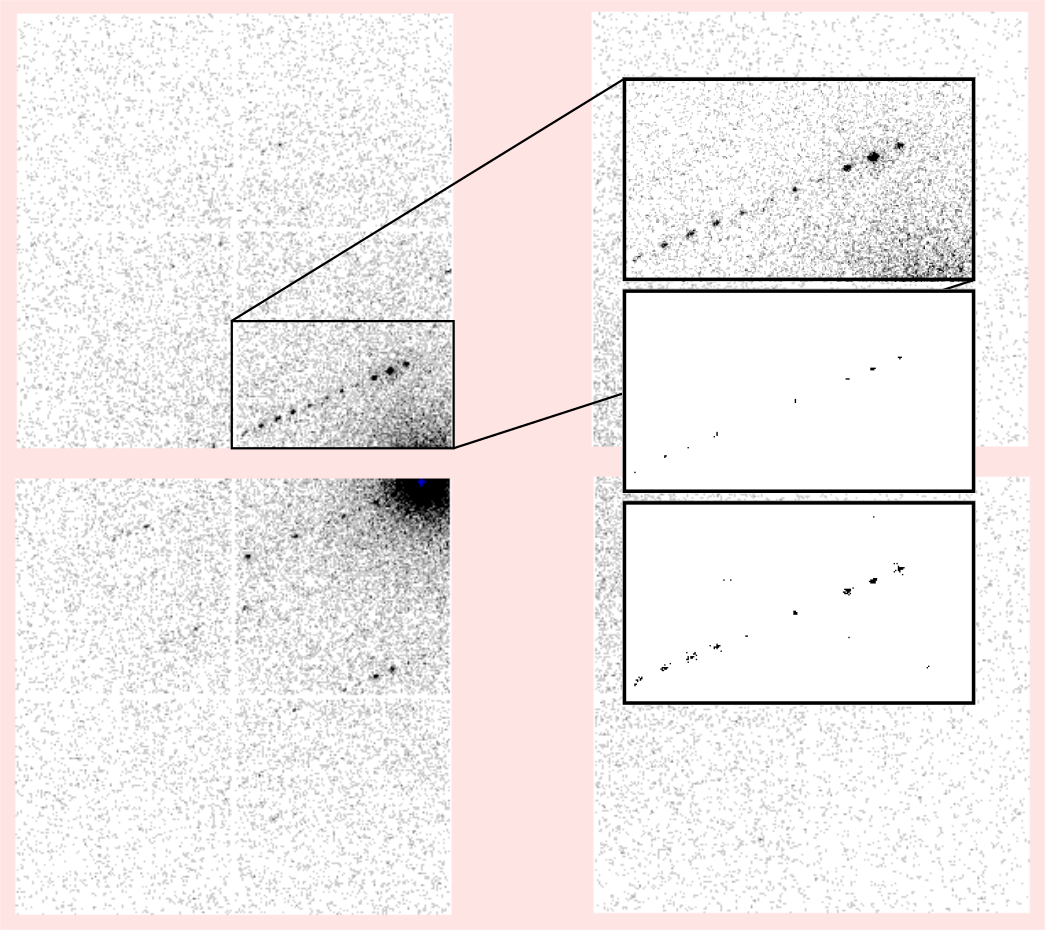
\includegraphics[width=0.5\textwidth]{Figures/spotfinding/spot_finding.png}
\end{figure}

\begin{figure}
  \label{fig:ewald}
  \centering
  \caption{
    The Ewald construction for the electron diffraction and the X--ray cases are
    compared. The cross-hatched circle represents the reciprocal lattice within
    a limiting sphere of $\SI{1}{\angstrom}$ resolution. The Ewald
    sphere for 12 keV X--rays with a wavelength of $\SI{1.0332}{\angstrom}$ is
    represented as a complete circle, with the scattering vector $\vec{s}_1$
    drawn at the $\SI{1}{\angstrom}$ limit, forming an angle of
    $2\theta_X=62.2^\circ$ from the incident beam direction along $\vec{s}_0$.
    At this scale, the Ewald sphere for 200 keV electrons, with a wavelength of
    $\SI{0.02508}{\angstrom}$ cannot be shown as a complete circle as it has
    radius of over forty times greater. The equivalent scattering vector
    $\vec{s}_1$ for $\SI{1}{\angstrom}$ diffraction forms an angle of only
    $2\theta_e=1.44^\circ$ from the incident beam direction. It is worth noting
    that reciprocal lattice is sampled along an almost planar surface,
    implying that data from a single image contains no information about the
    reciprocal lattice dimension in the direction along the incident beam.
  }
  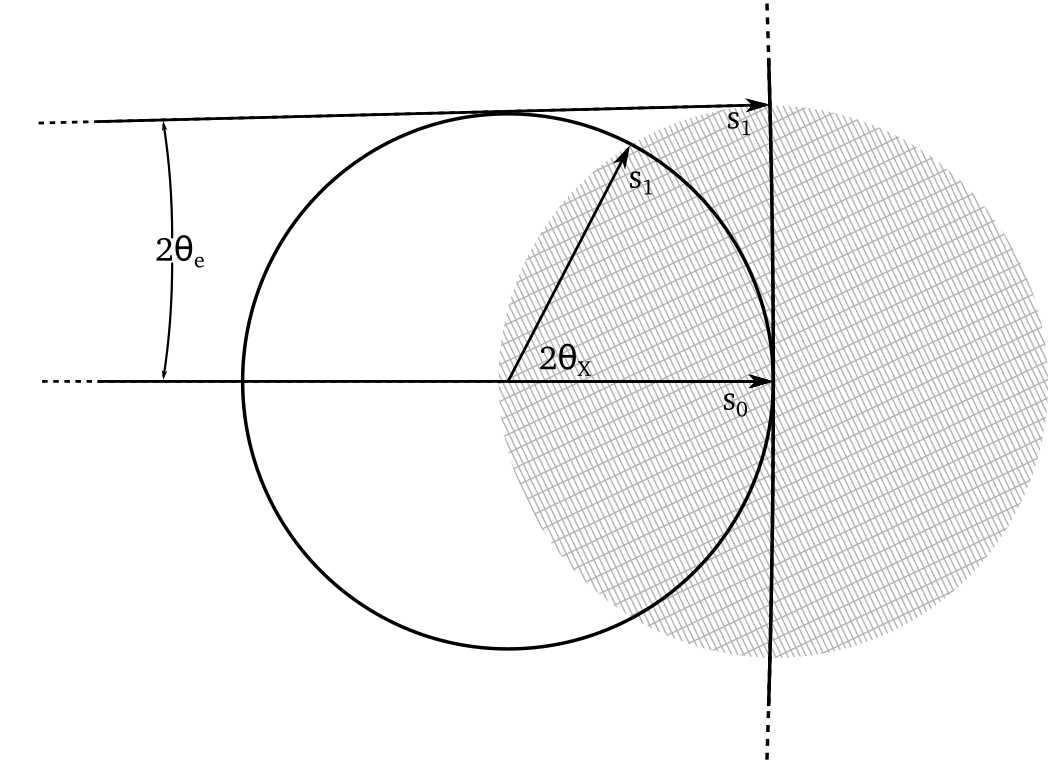
\includegraphics[width=0.5\textwidth]{Figures/geometry/ewald.png}
\end{figure}

\begin{figure}
  \label{fig:invert_axis}
  \centering
  \caption{
    Five reciprocal lattice points are shown (in black and labelled) along the
    $a^*$ axis for a crystal with unit cell dimension $a=\SI{10}{\angstrom}$.
    Arcs representing the surface of the Ewald sphere with a typical X-ray
    wavelength of $\lambda=\SI{1.0332}{\angstrom}$ intersect these points at
    rotation angles between $15.0^\circ$ for $h=1$ to $27.0^\circ$ for $h=5$,
    where rotations are assumed to be clockwise from vertical in the plane of
    the figure. If the modelled rotation axis is inverted then $\phi$-centroids
    of observed spots would be mapped onto Ewald spheres rotated between
    $-15.0^\circ$ and $-27.0^\circ$, resulting in a distinct curvature to the
    reconstructed reciprocal lattice (points shown in blue). In the case of
    electron diffraction at $\lambda=\SI{0.02508}{\angstrom}$ the spots are
    almost observed simultaneously, at rotation angles between $12.1^\circ$ and
    $12.4^\circ$. For clarity a single Ewald arc is shown, for $h=3$. If the
    assumed axis is inverted then $\phi$-centroids between $-12.1^\circ$ and
    $-12.4^\circ$ still result in almost a straight line (points shown in
    green). It is therefore difficult to determine the correct direction of
    rotation from the appearance of the reconstructed reciprocal lattice alone.
  }
  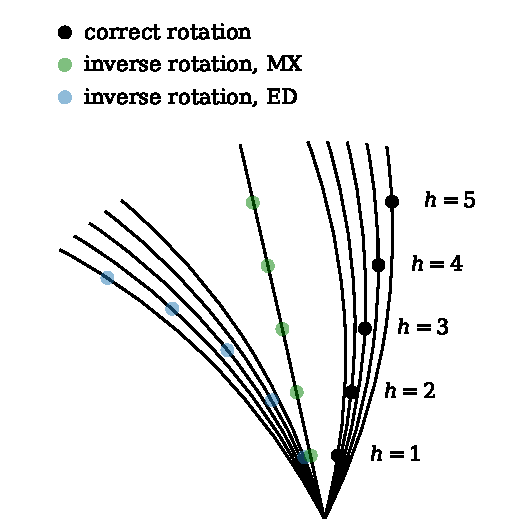
\includegraphics[width=0.5\textwidth]{Figures/relps_inverted_axis.pdf}
\end{figure}

\begin{figure}
  \label{fig:corrgram}
  \centering
  \caption{
    Geometry refinement against simulated data was performed assuming either
    typical electron diffraction geometry or X--ray diffraction geometry, as
    described in the text. Corrgrams were produced for the final step of
    refinement. Here, corrgrams indicating the correlation between effects of
    different parameters on the angular residuals $(\phi - \phi_o)$ are shown,
    with the refined detector parameters excluded from the plots as they have
    no effect on the $\phi$ residuals. The parameter labels are as defined in
    \citeasnoun{Waterman2016}. The upper panel shows the corrgram for the
    electron diffraction geometry and the lower panel shows the equivalent for
    the X--ray diffraction geometry.
  }
  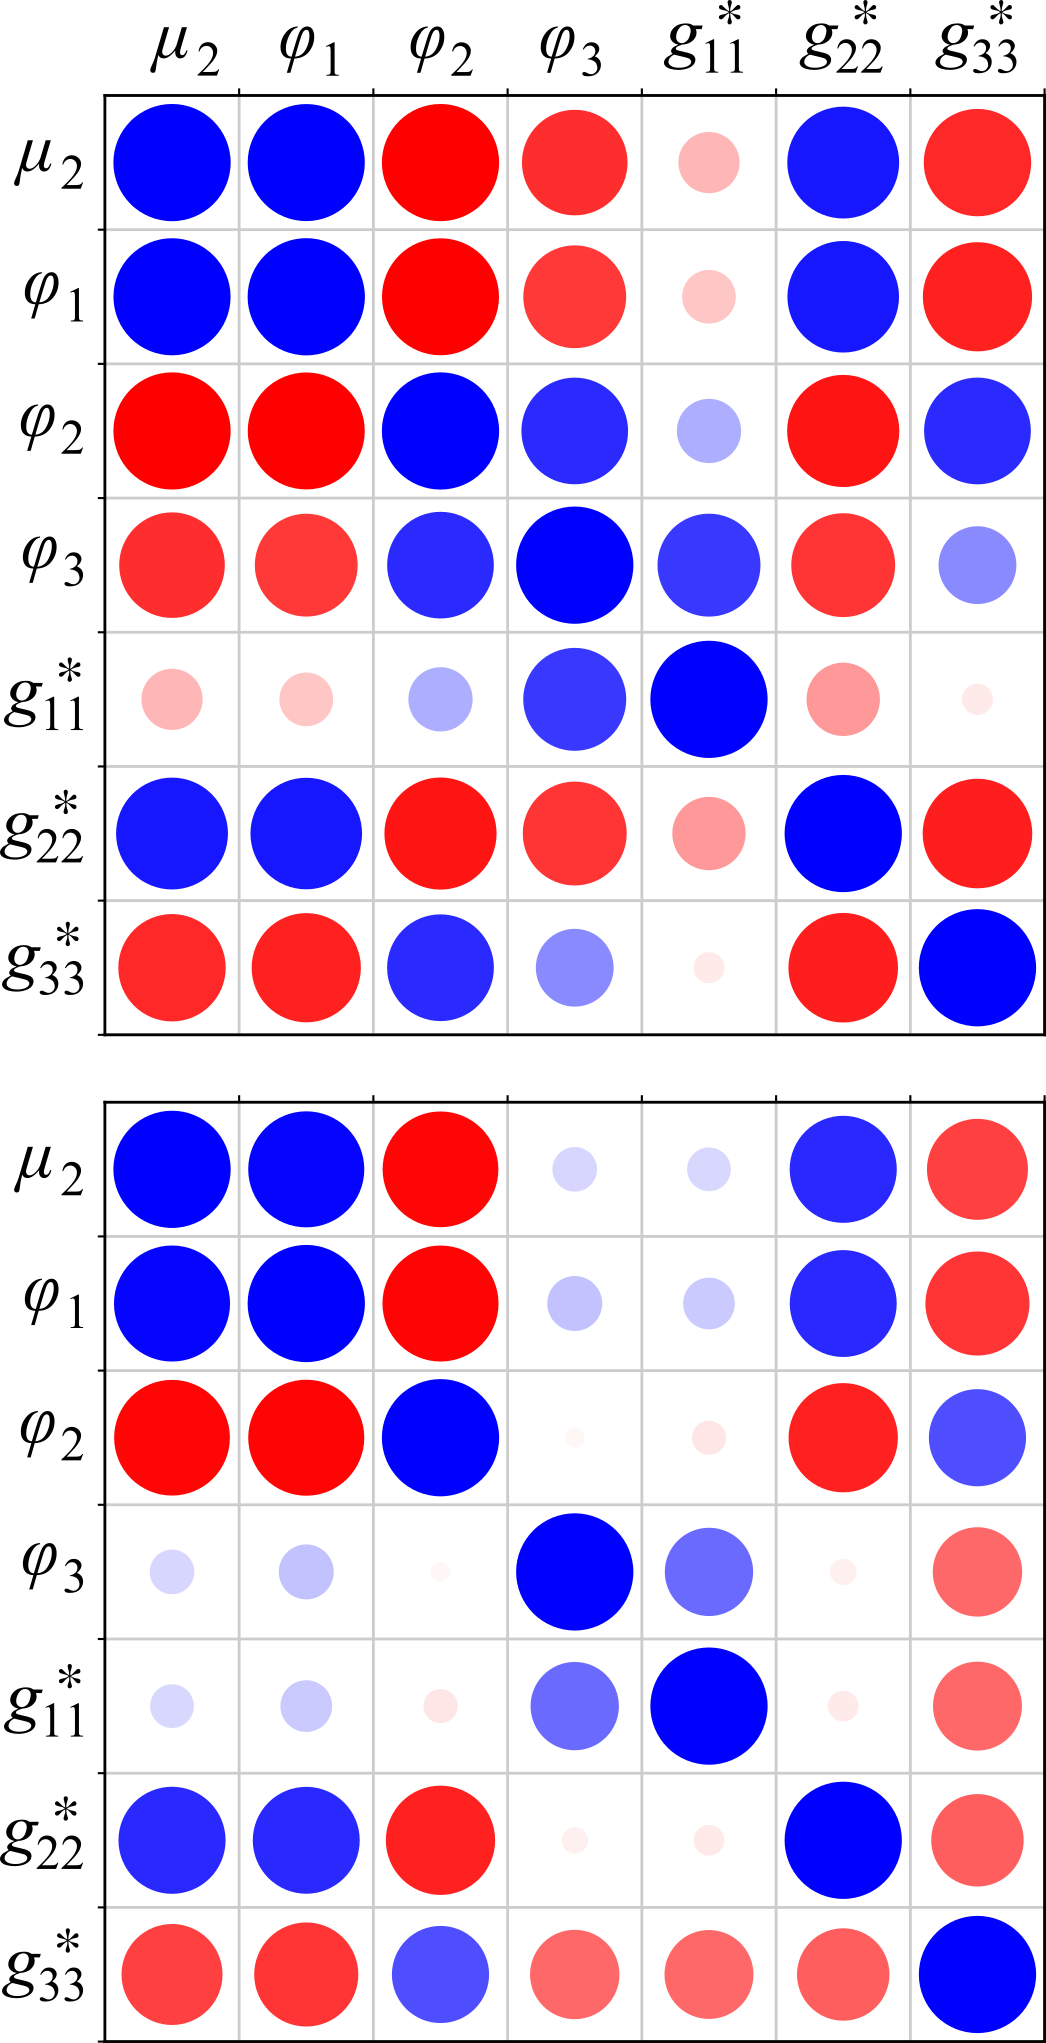
\includegraphics[width=0.5\textwidth]{Figures/simulation/corrgrams_phi.png}
\end{figure}

\appendix

\section{\code{PHIL} examples \label{app:PHIL_example}}

The following options were written to a file, which was passed to \dialsimport
in order to override the initial model for experimental geometry of the example
\emph{dataset 1}.

\begin{verbatim}
geometry.scan.oscillation=0,0.076
geometry.goniometer.axes=-0.018138,-0.999803,0.008012
geometry.detector.hierarchy{
  fast_axis=1,0,0
  slow_axis=0,-1,0
  origin=-26.3525,30.535,-1890
}
\end{verbatim}

Unit cell restraints to an external target cell were created for
\emph{dataset 6} of
the example set by writing the following lines to a file and passing this in
at \dialsindex and \dialsrefine steps.

\begin{verbatim}
refinement
{
  parameterisation
  {
    crystal
    {
      unit_cell
      {
        restraints
        {
          tie_to_target
          {
            values=32.05,68.05,104.56,90,90,90
            sigmas=0.05,0.05,0.05,0.05,0.05,0.05
          }
        }
      }
    }
  }
}
\end{verbatim}

The correct format for these options may be explored interactively using
command line switches for \dials programs. For example, the command
\texttt{dials.import -c -a2 -e2} will show all configuration options along with
types and help strings up to an `expert level' of 2.

\section{Simulation for comparison of ED versus MX geometry refinement
  \label{app:simulation}}
\DW{This may move to supplementary material rather than an appendix}

To generate simulated spot centroid positions, we started with the real electron
diffraction example \emph{dataset 1}, consisting of a continuous rotation scan over 503 images with
an angular width of $0.076^\circ$ per image, for a total scan range of
$38.2^\circ$. We took the model for the indexed experiments and ``regularised''
the geometry of the beam and detector for the purposes of simulation, without
changing the crystal model, which had an orthorhombic unit cell with dimensions
$a=\SI{31.97}{\angstrom}$, $b=\SI{69.41}{\angstrom}$ and
$c=\SI{104.62}{\angstrom}$. To regularise the beam and detector models, we
forced the beam direction to be exactly aligned to the $-Z$ direction and
reoriented the detector model such that the beam intersected the detector in
the centre of its square window, and the detector plane was orthogonal to the
beam vector. The detector distance remained at the value of
$\SI{1890}{\milli\metre}$, as previously determined and stored in the CBF headers
for the images. The real detector consists of $2\times2$ Timepix quads with
large gaps between the active regions. For simplicity we replaced this model
with a single panel covering the total extent of the real detector, with
no parallax correction, effectively assuming it consists of a perfectly
sensitive plane of zero thickness. The updated electron diffraction geometry
was written to a new \dxtbx experiment list and then altered a second time to
produce regularised geometry for an X-ray experiment. This involved changing
the wavelength from $\SI{0.02508}{\angstrom}$ to $\SI{1.0332}{\angstrom}$ and the
detector model such that the total extent and pixel size was equivalent to a
Pilatus 6M detector at a distance of $\SI{200}{\milli\metre}$ from the sample.
This model was also written to a \dxtbx experiment list. The differences
between the model geometries are shown in Table~\DW{Table: diffraction geometry
simulation models}.

The regularised models were used alongside the indexed spot list from the
real data set to simulate observed centroid positions for both versions of the
experimental geometry. By using the spot list from a real experiment we ensured
a realistic distribution of strong spots versus resolution. In order to ensure
that the differences in refinement runs are caused only by the
diffraction geometry and not obscured by different sets of input spots, we
selected 1571 reflections that could be predicted by both versions of the
diffraction geometry.

Simulated centroid positions were calculated for each version of the geometry
by predicting their positions then adding random error. The random errors were
drawn from a normal distribution with a standard deviation of 0.25 pixels for
the $X$ and $Y$ positions and 0.25 images for the $Z$ position. For real data,
the centroid position errors in $X$, $Y$ and $Z$ are neither independent, nor
normally-distributed. However, the purpose of adding displacements to the
centroid positions was merely to ensure that refinement would proceed to
convergence with realistic final RMSDs. The centroid positions from
spot-finding result from a centre-of-gravity calculation, which also provides
estimated errors in these positions that are used to set weights in
refinement. These errors have a dependence on the found spot intensity. Rather
than simulating new error estimates, we kept the original error
estimates from spot-finding on the real data set to give a realistic
distribution of weights. The centroid $X$, $Y$ positions and their errors were
rescaled to units of millimetres for use in refinement using the pixel sizes
shown in Table~\DW{ref Table above: diffraction geometry simulation models}.

\DW{Supplementary figure: all corrgrams}

\end{document}
